\documentclass[11pt]{article}
\usepackage[utf8]{inputenc}
\usepackage[T1]{fontenc}
\usepackage{graphicx}
\usepackage{longtable}
\usepackage{float}
\usepackage{wrapfig}
\usepackage{soul}
\usepackage{amssymb}
\usepackage{hyperref}
\usepackage[spanish]{babel}
\usepackage{bookman}
\usepackage[left=3cm,top=3cm,right=2cm,bottom=1cm,head=1.5cm,includefoot]{geometry}
\usepackage{listings}
\usepackage{multirow}
\usepackage{amssymb}
\usepackage{fancyhdr}
\usepackage{comment}
\usepackage{color}
\usepackage{multicol}
\usepackage[table]{xcolor}
\usepackage{ulem}

\title{informe}
\author{}

\begin{document}

% ---------------------- Encabezado y pie de página -----------------------

% Encabezado: sección a la derecha.
% Pie de página: número de página a la derecha.

\pagestyle{fancy}
\renewcommand{\sectionmark}[1]{\markboth{}{\thesection\ \ #1}}
\lhead{}
\chead{}
\rhead{\rightmark}
\lfoot{}
\cfoot{}
\rfoot{\thepage}


% Hago que las páginas se comiencen a contar a partir de aquí.
\setcounter{page}{1}

% Índice
\tableofcontents
\newpage


\section{Enunciado}

\begin{center}
% Orden del trim = izq abajo derecha arriba
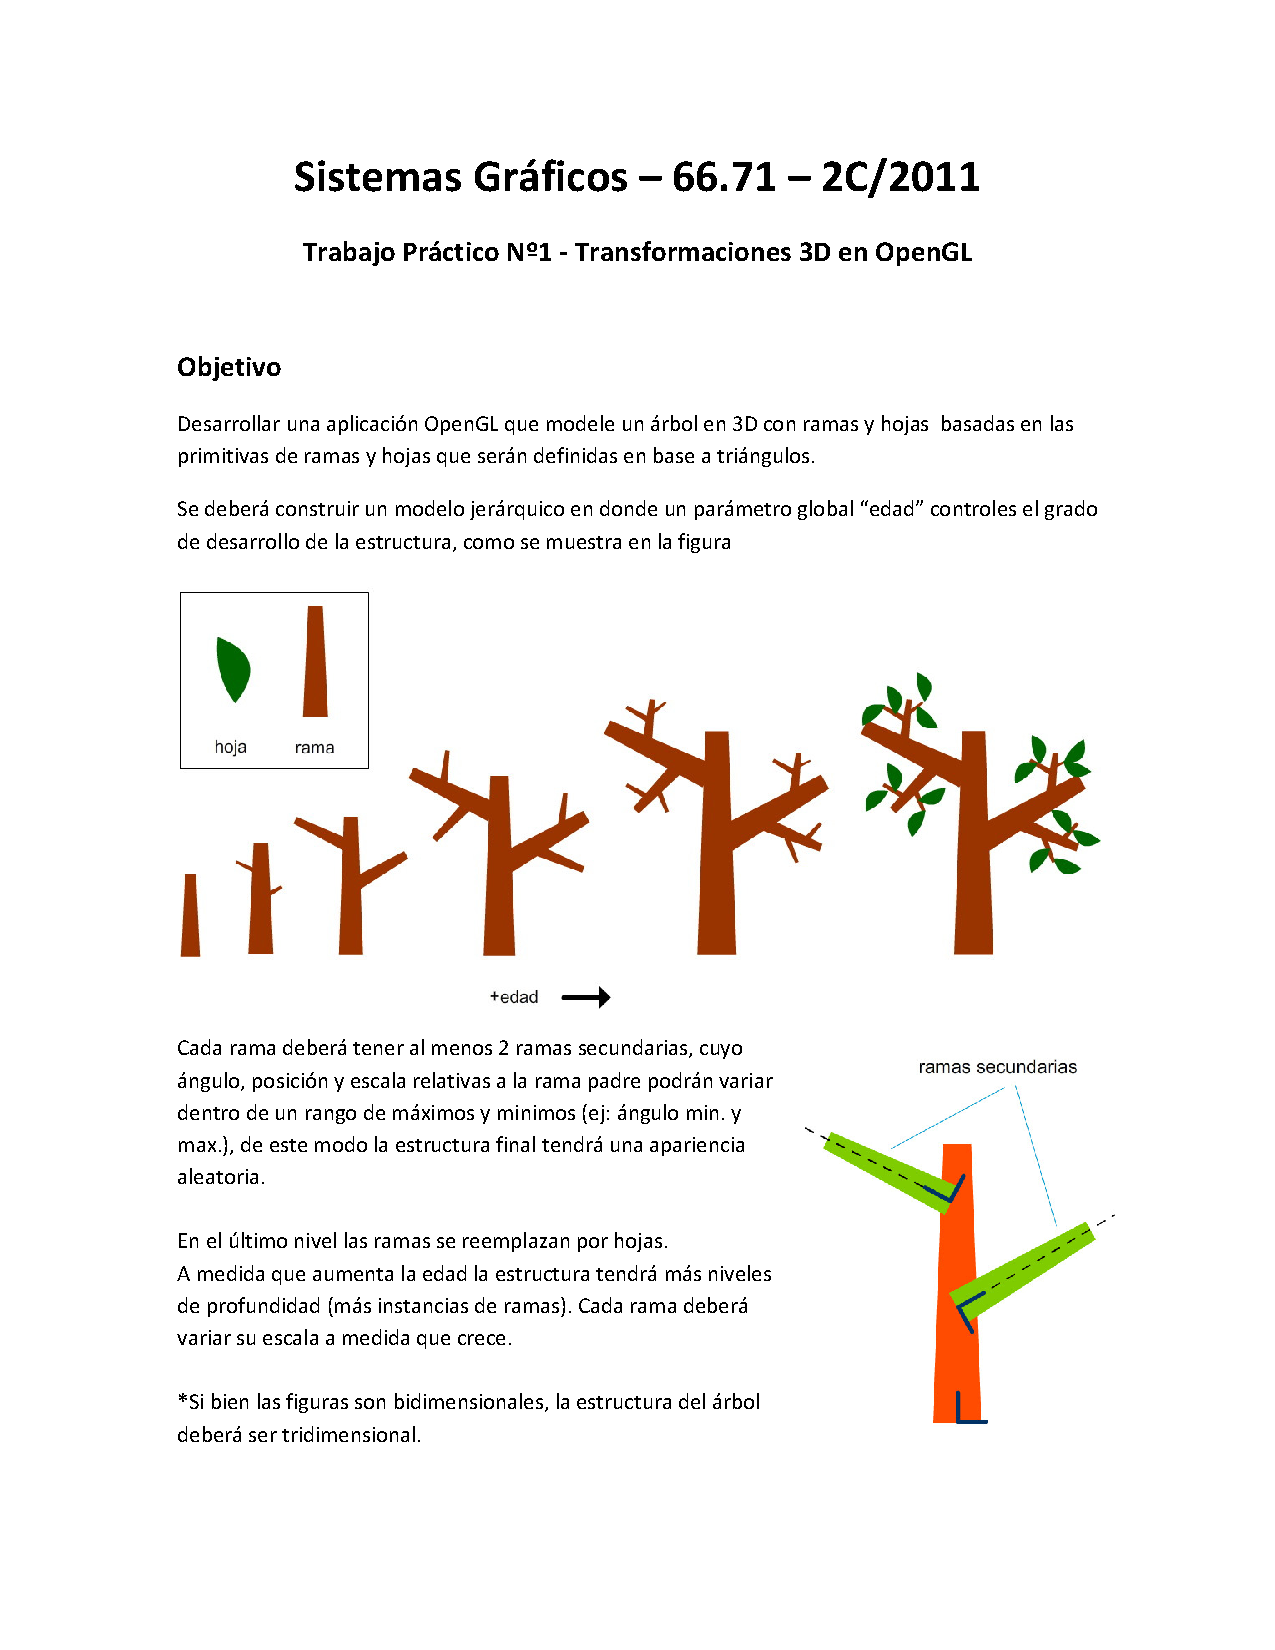
\includegraphics[trim = 25mm 30mm 10mm 35mm, clip,height=0.93\textheight,width=1.04\textwidth]{tp1-c2-2011.pdf}
\includegraphics[trim = 25mm 20mm 10mm 40mm, clip,height=0.95\textheight,width=1.04\textwidth,page={2}]{tp1-c2-2011.pdf}
\end{center}

\newpage


\section{Consideraciones de Dise\~no}
  El presente trabajo pr\'actico se basa en la utilizaci\'on de un algoritmo recursivo para dibujar y simular el crecimiento del \'arbol.
Este algoritmo, dibuja en cada llamada una rama, o en su defecto una hoja, de un determinado nivel del \'arbol. \\
  Para realizarlo, se tomaron en cuenta las siguientes consideraciones de dise\~no:
\begin{itemize} 
 \item Cada rama posee cuatro ramas hijas; o en su defecto cuatro hojas si se tratara del ante\'ultimo nivel. 
 \item Por defecto, el \'arbol tiene ocho niveles. Para modificar la cantidad de niveles, se puede pasar por l\'inea de comandos el par\'ametro con dicha cantidad. 
Se recomienda no exceder la cantidad de 10 niveles.
 \item La altura de cada nivel del \'arbol depende en forma cuadr\'atica de dicho nivel. La misma se actualiza aut\'omaticamente 
con el paso del tiempo, de forma tal de producir la sensaci\'on de que el \'arbol va creciendo hasta alcanzar su edad tope. Se consideraron 10
intervalos de tiempo para lograr que una rama en particular alcance su altura total.
 \item El di\'ametro de cada rama depende linealmente de la altura de la misma.
 \item Para dibujar las hojas se utilizaron dos tri\'angulos, empleando GL\_TRIANGLE\_STRIP, de forma tal de que los mismos conformen un rombo.
 \item Con el fin de dibujar el tronco y las ramas, se utilizaron tri\'angulos para conformar un cono truncado, junto con sus tapas.
 \item El \'angulo de una rama respecto de su hija var\'ia en funci\'on del nivel y en los rangos: [40; 40+NivelM\'aximo] y [30; 30+NivelM\'aximo ]; correspondiendo
 el mayor \'angulo a las ramas ubicadas a menor altura en la rama padre.
 \item Despu\'es de dibujar cada nivel, se realiza una rotaci\'on de 90 grados, de forma tal de lograr repartir las ramas en todo el espacio.
\end{itemize}

Asimismo, para el manejo de la c\'amara, se tomaron las siguientes consideraciones de dise\~no:
\begin{itemize} 
 \item Se puede hacer orbitar la c\'amara alrededor del \'arbol utilizando la tecla z y Z o presionando la tecla c para capturar el movimiento del mouse y rotar la camara con el mismo.
\item Se permite acercar la c\'amara hasta el tronco del \'arbol utilizando la tecla + y alejarse del mismo utilizando la tecla -.
\end{itemize}


\section{Compilaci\'on}
  Para compilar la aplicaci\'on bajo entorno Linux se provee un archivo de makefile.
  Para utilizar el mismo, debe tenerse instalada la herramienta cmake. Para instalarla, por ejemplo, en una distribuci\'on Ubuntu se deben 
realizar los siguientes pasos: \\
1) sudo apt-get install cmake \\
2) Ingresar la contrase\~na de root del usuario. \\
3) Aceptar la descarga e instalaci\'on de los paquetes necesarios. \\ 

Teniendo ya instalada la herramienta, posicionados en el directorio donde se encuentra el trabajo pr\'actico es necesario crear un directorio build
de la siguiente forma: \\
mkdir build \\
cd build \\
cmake .. \\
make \\

Una vez realizados estos pasos, se dispondr\'a del ejecutable de nombre tp1.

\section{Ejecuci\'on}

Para ejecutar la aplicacio\'n bajo un entorno Linux se deben realizar los siguientes pasos: \\
1)Posicionarse en el directorio build creado anteriormente. \\
2)Ejecutar: \\
./tp1 


\section{Controles de teclado}

La aplicaci\'on permite realizar las siguientes acciones utilizando las teclas detalladas a continuaci\'on: \\


    \begin{tabular}{|| l | l ||}
      \hline
      \begin{large}Tecla\end{large} & 
	\begin{large}Acci\'{o}n \end{large} \\
          \hline
R & Reiniciar la animaci\'on de crecimiento \\
P & Pausar/reanudar la animaci\'on  \\
Q & Incrementar la velocidad de crecimiento  \\
A & Decrementar la velocidad de crecimiento  \\
q & Salir de la aplicaci\'on  \\
a & Muestra/esconde los ejes  \\
g & Muestra/esconde la grilla  \\
c & Captura/libera el movimiento del mouse para rotar la c\'amara  \\
z & Rotar la c\'amara alrededor del \'arbol en sentido antihorario  \\
Z & Rotar la c\'amara alrededor del \'arbol en sentido horario  \\
+ & Acercar la c\'amara al \'arbol  \\
- & Alejar la c\'amara del \'arbol  \\

          \hline
    \end{tabular}



\end{document}

